\chapter{Local Flags}

In the previous chapter we saw how to use flag algebras to bound density functions
asymptotically, Some things are not described by a density function but still feel
"density like", leading us to speculate if we can modify the flag algebra method to work
for these functions.

For example, in chapter TODO we will see a problem we're calling the bounded degree
Erd\H{o}s' pentagon problem. In approaching that problem we will ask:
Given a triangle-free graph $G$ with max degree $\Delta(G)$ and some fixed vertex
$v\in V(G)$, how many pentagons (5-cycles) are there containing $v$?
We want to upper bound this number of pentagons as a function of $\Delta(G)$. The upper
bound of $\Delta(G)^4$ is easily seen, but $\frac{1}{2}\Delta(G)^4$ is also easy to prove.

Phrased differently: If $f(G)$ is the number of pentagons in $G$ containing $v$ then
we want to find an asymptotic upper bound on $f(G) / \Delta(G)^4$. If we pick a
flag $F=\cfivemarked$ which is a pentagon with a single labelled vertex then this
could be written as $c(F; G^v) / \Delta(G)^4$.

This looks a lot like
a density function, except that our denominator is of the wrong form: It should
be $\in\Theta(|G|^4)$, not $\Delta(G)^4$. It is for this reason that applying classic
flag algebras directly is not promising: Our function is of the wrong form. We will
see in section TODO that a few ways we could try and "trick" the density function do not
work out.

It turns out though that we can define a new type of "density function" which
can be used to bound functions like $c(F; G^v) / \Delta(G)^4$. These density functions
then also have a rich (but notably limited) algebraic structure which we can exploit.

In the following sections we introduce our new local density function and then go on to
define local versions of many of the same structures that exist in the classic flag
algebra. We then prove the algebraic structure these \textit{local flags} possess.

\section{Local Flags}

Let $\Gcl$ be some graph class as before\footnote{We assume here $\Gcl$ is hereditary but we will address later that it may not be}.
Let $\Delta$ be some graph parameter $\Delta\colon \Gcl \to \N_0$
such that $\Delta(G)\to\infty$ implies $|G|\to\infty.$
(More formally there is some monotone increasing
unbounded function $f$ such that for all $G\in\mathcal{G}$ we have $|G|\geq f(\Delta(G))$).


\begin{note}
    We almost exclusively use the maximum degree function $\Delta$ so you can effectively always
    interpret $\Delta(G)$ in this way. Clearly $|G|\geq\Delta(G)$. In particular all of
    our examples use the max degree function for $\Delta(G)$.
\end{note}

We start by defining the \textit{local density} in the same way as the induced
density (Definition \ref{def:induced_density}) but with a different denominator.
We use the definition of $\sigma$-flags (Definition \ref{def:sigma_flag}) from the
classic flag algebras directly.

\begin{definition}[Local Density]
    Let $(F, \theta), (G,\eta)$ be $\sigma$-flags as before. Then $c((F,\theta), (G,\eta))$ is
    the induced count (Definition \ref{def:induced_count}). Define the
    \textbf{local density} $\rho((F, \theta), (G, \eta))$ to be
    \[
        \rho(F; G) := \frac{c(F; G)}{\binom{\Delta(G)}{|F|-|\sigma|}}.
    \]
    Note the $\rho \neq p$ notation.
\end{definition}

Because of our choice of normalisation we are not
guaranteed the $[0,1]$ codomain as in the classic case. In particular this
destroys the nice probabilistic sampling interpretation that we had with the
induced density function. In general this function may be bounded or unbounded:

\begin{example}
    If $\Gcl$ is all graphs then $c(\vertex; G)= |V(G)|$ hence
    $\rho(\vertex; G) = \frac{|G|}{\Delta(G)}$ which is an unbounded function.
\end{example}

\begin{example}
    If $\Gcl$ is all graphs then consider the $\vertex$-flag $\edgemarked$. Then for
    any $G$ with distinguished vertex $v$ we have $c(\edgemarked; G^v)=\deg(v)$
    so $\rho(\edgemarked; G^v) = \frac{\deg v}{\Delta(G)} \leq 1$.
\end{example}

This bounded/unbounded distinction is the key distinction we want to make. Those
flags $F$ with bounded behaviour are those with the exploitable algebraic structure. Indeed
we will eventually define our \textit{local flags} to be those with bounded local density
but we first need to address some technical definitions to avoid pathological cases:

We need a way to technically describe the action of taking a $\sigma$-flag with some
unlabelled vertices and labelling one of those vertices:

\begin{definition}[Label Extension]
    Given a $\sigma$-flag $(F, \theta)$ and some $v\in V(F)$ which is unlabelled
    ($\notin\im\theta$) we can construct a \textbf{label extension}
    $\theta'\colon [|\sigma|+1] \to V(F)$ as
    \[
        \theta'(i) = \begin{cases}
            \theta(i) & \text{if}\ i\in[|\sigma|]\\
            v & \text{otherwise}
        \end{cases}
    \]
    This is an embedding of the type $\sigma'$ obtained by adding new vertex $|\sigma|+1$
    to $\sigma$ such that $\sigma' \cong F[\im \theta \cup \{v\}]$. See figure
    \ref{fig:labelling_ext_example} for an example of a flag and all its possible label
    extensions.
\end{definition}

\begin{figure}[ht]
    \centering
    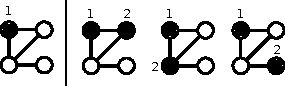
\includegraphics[scale=1.5]{labelling_ext_example.pdf}
    \caption{All possible label extensions of a flag}
    \label{fig:labelling_ext_example}
\end{figure}

The other technicality we need to address is that of the hereditary nature of graph
classes. In the classic flag algebra we always assumed that $\Gcl$ was hereditary. We want
to be able to talk about some non-hereditary graph classes $\Gcl$. This is not a major
obstacle but means we need to adjust our notation.

\begin{definition}[Hereditary Closure]
    Given a graph class $\Gcl$ we define the \textbf{hereditary closure} of $\Gcl$ to be
    the smallest graph class which contains $\Gcl$ and is closed under taking
    induced subgraphs. i.e. it's the graphs $G\in\Gcl$ with their induced subgraphs.

    We denote this as $\HeredG$.
\end{definition}

Now we are ready to define our local flags:

\begin{definition}[Local $\sigma$-Flag]
    Fix some graph class $\Gcl$ and takes its hereditary closure $\HeredG$.
    Let $\sigma$ be a type. Then a $\sigma$-flag $(F, \theta)\in\HeredG{}^\sigma$ is a
    \textbf{local $\sigma$-flag} if we have the following properties:
    \begin{enumerate}
        \item $(G,\eta) \to \rho((F,\theta); (G,\eta))$ is a bounded function as a function
            $\Gcl^\sigma\to\R_{\geq 0}$. (We are very intentionally using $\Gcl$ and not its closure here).
        \item If we label any of $F$'s unlabelled vertices we get another local flag.
    \end{enumerate}
\end{definition}

To state this 2nd property more precisely: We require that for any label extension
$\theta'$ of $\theta$, the induced extended flag $(F,\theta')$ is also a local flag.
This is not a circular definition as any label extension of $(F,\theta)$ reduces the number of
unlabelled vertices
by 1; We could define inductively starting with those flags with no unlabelled vertices.

What we're trying to capture here is that any "subflag"
of $F$ is also a local flag, meaning we can pin down
$F$'s vertices and continue to get bounded behaviour.

\begin{example}
    As in the example above $F=\edgemarked$ gives rise to a bounded local
    density function $\rho$. The only label extension of $F$ is the edge
    with both vertices labelled $F' = \edgebothmarked$. This (as with all flags with no
    unlabelled vertices) has $c(F'; G) = 1$ so $\rho(F; G) = 1/\binom{\Delta(G)}{0}=1$
    which is bounded so $F'$ is a local flag. Hence $F=\edgemarked$ is a local flag.
\end{example}

We write $\Glocn^\sigma\subseteq\HeredG{}^\sigma_n$ for the set of local $\sigma$-flags
of size $n$ up to isomorphism, and $\Gloc^\sigma$ for all local $\sigma$-flags. As usual we
can drop the $\sigma$ superscript if $\sigma=\emptyset$.

Comparing this section to the classic flag algebra case (section \ref{sec:flag_algebras})
you might expect us to introduce something akin to the chain rule (lemma \ref{lemma:chain_rule}).
Unfortunately no such relation exists in general for local flags. This is the first big
loss when moving to the new framework: Prima facie it's unclear how one can "project"
small flags into the space of larger flags.

\begin{note}
    This second property we require of local flags is not necessarily implied by
    the first which we show now in lemma \ref{lemma:second_prop_required}.
\end{note}

\begin{lemma}
    \label{lemma:second_prop_required}
    There is a class of graphs $\Gcl$ and $\sigma$-flag $F$ such that
    $G \mapsto \rho(F; G)$ is a bounded function $\Gcl^\sigma \to \R$ but $F$ is
    not a local $\sigma$-flag. i.e. $F$ has a labelled extension with unbounded
    density function.
\end{lemma}
\begin{proof}
    Take $\Gcl$ to be the class of 3-vertex-coloured graphs (black, red and blue) $G$
    which have a single red vertex and $\Delta(G)^2$ blue vertices\footnote{Implicitly the
    rest of the vertices are black} such that there are no edges between red and blue
    vertices.

    Then take $\emptyset$-flag $F=\redbluenonedge$. For any $G\in\Gcl$ we have
    $c(F; G) = \Delta(G)^2$ as there is 1 choice for the red vertex and $\Delta(G)^2$
    choices for the blue. Hence $\rho(F;G) = c(F; G) / \binom{\Delta(G)}{2} \leq 2$.
    Consider then the labelled extension $F' =\redbluenonedgemarked$ of type
    $\redvertex$. We have $c(F'; G)=\Delta(G)^2$ again for any
    $G\in\Gcl^\redvertex$ but now $\rho(F'; G) = \Delta(G)^2 / \Delta(G) = \Delta(G)$ which
    is an unbounded function. Hence $F'$ is not a local $\redvertex$-flag
    meaning $F$ is not a local $\emptyset$-flag.
\end{proof}

Intuitively $F$ is a local $\sigma$-flag (relative to our choice of $\Gcl$ and
$\Delta$) if $\Delta(G)$ bounds the "degree of freedom" for the possible mapping
of $F$'s unlabelled vertices. Consider the following example.

\begin{example}
    Let $\Gcl$ be the class of 2-vertex-coloured (black and red) graphs such that
    each $G\in\Gcl$ has $\leq \Delta(G)$ black vertices where as usual $\Delta(G)$ is the
    max degree of $G$.

    Take some connected graph $F$. If $F$ contains a black vertex then
    $F$ is a local $\emptyset$-flag:
    To see this take one of the black vertices in $F$.
    It must map to some black vertex in $G$, there are $\Delta(G)$ such choices.
    Then each vertex in $F$ connected to our black vertex must map into the neighbourhood
    of its image in $G$, which has size $\leq\Delta(G)$. This logic continues showing
    each vertex has at most $\Delta(G)$ possible images in $G$ leading to a bound of
    $c(F; G) \leq \Delta(G)^{|F|}$. The argument is almost identical for any labelled
    extension of $F$.

    Then in general connected components are independent of each other so we generalise
    to say that if each connected component of some $F$ contains a black vertex then
    $F$ is a local $\emptyset$-flag. We will see a more rigorous version of this
    argument in TODO REF.
\end{example}

\section{Algebraic Structure}

Now that we have described local $\sigma$-flags $\Gloc$ we can describe their
algebraic structure. Ideally we would like to construct a product structure
on $\Gloc$ such that we get a result like theorem \ref{thm:classic_product_lim} but for
local density function $\rho$. In fact this is exactly what we get: We will get an
algebraic structure such that $\rho(f; G)\rho(g;G) = \rho(f\cdot g; G) + o(1)$.

First we take the concept of limit functionals (section \ref{sec:limit_functionals})
from the classic flag algebras with some minor modifications:
First, we require now that a sequence of graphs $(G_k)_{k\in\N}$ is $\Delta$-increasing:
\begin{definition}
    A sequence $(G_k)_{k\in\N}$ is $\Delta$-increasing if the sequence
    $(\Delta(G))_{k\in\N}$ is strictly increasing\footnote{We required that the codomain of
    $\Delta$ was $\N$ so strictly increasing implies unbounded. Generalising $\Delta$
    to a function with codomain $\R$ is likely possible so we would need to add the
    unbounded requirement here.}.
\end{definition}
Then given some $\Delta$-increasing sequence of $\sigma$-flags $(G_k)_{k\in\N}$
and some local $\sigma$-flag
$F$ we can look at $\lim_{k\to\infty}\rho(F; G_k)$. As $F$ is a local $\sigma$-flag
$\rho(F; \cdot)$ is bounded so the image is compact. For this reason (again via Tychonoff's theorem)
any sequence of $\sigma$-flags $(G_k)_{k\in\N}$ contains a convergent subsequence meaning
$\lim_{k\to\infty}\rho(F; G_k)$ exists for all $F\in\Gloc^\sigma$.
Hence we can define a limit functional $\phi\colon\Gloc^\sigma\to\R$
from such a convergent sequence $(G_k)_{k\in\N}$ as $\phi(F)=\lim_{k\to\infty}\rho(F; G_k)$.

As with the classic case we can take the space of formal linear combinations of
local flags $\R\Gloc^\sigma$ and linearly extend $\rho$ and $\phi$ to these
spaces. As before we denote the set of all limit functionals on type $\sigma$ by
$\Phi^\sigma$.

\begin{note}
    Unlike in the classic case we will not be quotienting the space $\R\Gloc^\sigma$ by
    a subspace. This is as we do not have an equivalent relation like the chain rule.
    The side effect of this is that there may be vectors $f \in \R\Gloc^\sigma$ which
    are formally non-zero but have $\phi(f) = 0\ \forall\ \phi\in\Phi^\sigma$.

    This doesn't affect the correctness of our arguments, but does mean the semidefinite
    programs will be larger and therefore may take longer to solve.
\end{note}

We now define the product on $\R\Gloc^\sigma$ which will turn it into an algebra.

\begin{definition}[Local Flag Product]
    Let $F, F'\in\Gloc^\sigma$ be given. Let $n=|F|+|F'|-|\sigma|$, the minimum size of
    a flag which can fit $F$ and $F'$. Then we define:
    \[
        F \cdot F' := \sum_{H \in \Glocn^\sigma} p(F, F'; H) \cdot H
    \]
    Note: This is the induced density function $p$, not the local density function $\rho$.
    Extend this product bilinearly to the space $\R\Gloc^\sigma$ to create an algebra
    $\Lcl^\sigma$.
\end{definition}

\begin{lemma}
    The algebra $\Lcl^\sigma$ is associative, commutative and unital.
\end{lemma}

We will prove this later. First we need to see a key technical lemma which makes this
product work.

\begin{lemma}
    Let $F, F' \in \Gloc^\sigma$ be local $\sigma$-flags and $H$ a $\sigma$-flag
    of size $n=|F|+|F'|-|\sigma|$ such that $p(F, F'; H) > 0$ then $H$ is a local
    $\sigma$-flag.
\end{lemma}

\begin{proof}
    Let $\theta,\theta'$ be the $\sigma$ embeddings for $F, F'$ and $\eta$ the
    $\sigma$-embedding for $H.$

    To prove $H$ is a local flag we first need to show that $\rho(H; \cdot)$ is a bounded function.
    i.e. $(G \mapsto c(H; G)) \in O(\Delta(G)^{|H|-|\sigma|}).$

    As $p(F, F'; H) > 0$ there is some $U, U'\subseteq V(H)$ such that $U\cap U'=\im\eta$ and
    $F \cong H[U] \land F'\cong H[U']$ as $\sigma$ flags. As $|H|=|F|+|F'|-|\sigma$ we
    have $U \cup U' = V(H)$.

    Let $(G, \zeta)$ be another $\sigma$-flag. If $c(H; G) = 0$ we're done so assume otherwise and
    let $\im\zeta \subseteq V\subseteq V(G)$ be such that $H \cong G[V]$ as $\sigma$-flags. Let
    $\phi$ be this isomorphism. Then In particular $\phi$ induces an embedding of $U, U'$ into
    $V(G)$ such that $\im\zeta = \phi(U) \cap \phi(U')$ and $G[\phi(U)] \cong F\land G[\phi(U')]
    \cong F'$ as $\sigma$-flags.  Hence any choice of an instance of $G$ in $H$ and choice of
    instances $U, U'$ of $F, F'$ in $H$ gives rise to a pair of instances of $F$ and $F'$ in $G.$
    There are at most some constant number $C$ instances of $F, F'$ in $H$ (as the size of $H$ is
    fixed).

    Note then also that any choice of a pair of instances of $F, F'$ in $G$ can be derived from at
    most 1 instance of $H$, as the size of $H$ was chosen to be the minimum possible such that both
    $F,F'$ fit. If the two instances overlap (outside of the required intersection at $\im\zeta$)
    then they don't correspond to an instance of $H.$ If they don't overlap then their
    union corresponds to a single \textit{possible} instance of $G.$

    In summary each instance of $H$ gives rise to some non-zero but bounded number of pairs of
    instances of $F, F'$ in $G$, and each pair of instances is induced by at most 1 instance of $H.$
    Therefore $c(H; G) \leq \frac{1}{C}\cdot c(F; G)\cdot c(F'; G).$ $c(F; \cdot)$ and
    $c(F', \cdot)$ are $\in O(\Delta(G)^{|F|-|\sigma|})$ and $\in O(\Delta(G)^{|F'|-|\sigma|})$
    respectively as $F,F'$ are local flags hence their product is
    $\in O(\Delta(G)^{|F|+|F'|-2|\sigma|}) = O(\Delta(G)^{|H|-|\sigma|})$ so
    $c(G, \cdot) \in O(\Delta(G)^{|H|-|\sigma})$ showing $\rho(G, \cdot)$ is a bounded function as
    required.

    TODO DIAGRAM

    It remains to prove that $H$ still has bounded density after fixing any unlabelled vertices.
    TODO
\end{proof}
